\label{appendix:moseg_additional_results}

\subsection{Motion Segmentation additional ATE results}
In this section, additional results for the Motion Segmentation system
to complement those outlined in Section~\ref{sec:moseg_quantitative} are given.
The results in this section assess Absolute Trajectory Error on the TUM Dynamic
Objects \textit{Validation} set. Quantitative results are given in Table
~\ref{tbl:moseg_ate_validation} and visualised in Figure
~\ref{fig:moseg_ate_validation}.

\begin{table}[h]
  \label{tbl:moseg_ate_validation}
\begin{center}
  \begin{tabular}{l@{\hskip 1cm} c c}
    \emph{TUM Standard Sequence Name} & \emph{MoSeg} ATE & \emph{Baseline} ATE \\
    \midrule
    \textsf{fr3-sitting-static} & 0.046 \std{0.021} & \textbf{0.030 \std{0.014}}\\
    \textsf{fr3-sitting-xyz} & 0.048 \std{0.027} & 0.048 \std{0.027}\\
    \textsf{fr3-sitting-halfsphere} & 0.029 \std{0.013} & \textbf{0.028 \std{0.012}}\\
    \textsf{fr3-sitting-rpy} & 0.047 \std{0.022} & \textbf{0.044 \std{0.020}}\\
    \textsf{fr3-walking-static} & \textbf{0.163 \std{0.191}} & 0.466 \std{0.252}\\
    \textsf{fr3-walking-xyz} & \textbf{0.092 \std{0.075}} & 0.633 \std{0.429}\\
    \textsf{fr3-walking-halfsphere} & \textbf{0.412 \std{0.271}} & 0.525 \std{0.325}\\
    \textsf{fr3-walking-rpy} & \textbf{0.082 \std{0.042}} & 0.561 \std{0.182}\\
  \end{tabular}
\end{center}
\caption[Motion Segmentation ATE Validation Set]
{The Absolute Trajectory Error (ATE) results (in metres, lower is better
  ) achieved by the proposed approach in comparison to the baseline InfiniTAM
 ~\cite{Prisacariu2014} framework on a variety of the standard sequences from
  the TUM RGBD \textit{Validation} dataset~\cite{Sturm2012}. Results are in the
  format mean $\pm$ standard deviation. The better result (by mean) on each
  sequence is highlighted in bold.}
\end{table}

\begin{figure}[h]
  \label{fig:moseg_ate_validation}
  \centering
  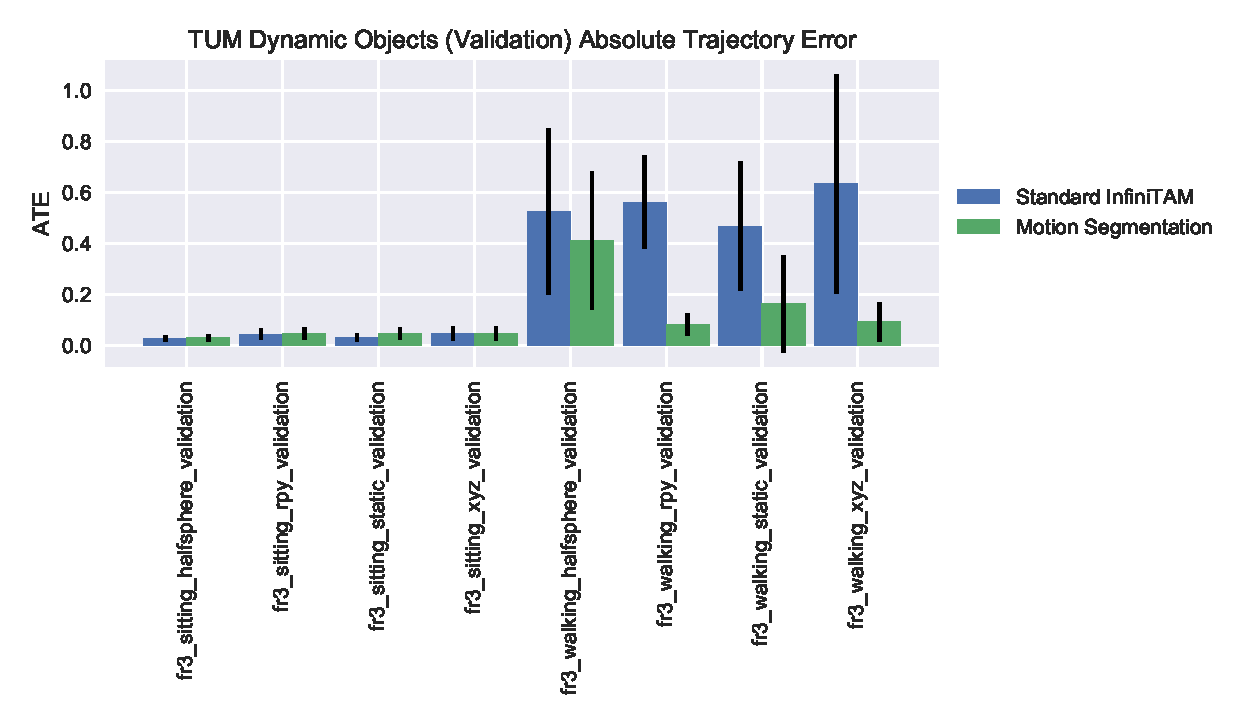
\includegraphics[width=\linewidth]{figures/moseg/ate_validation.eps}
  \caption[Motion Segmentation ATE Validation Set]
  {Absolute Trajectory Error for the TUM Dynamic Scenes
    \textit{Validation} dataset.}
\end{figure}

\subsection{Motion Segmentation additional RTE results}
In this section, additional results for the Motion Segmentation system
to complement those outlined in Section~\ref{sec:moseg_quantitative} are given.
The results in this section assess Relative Trajectory Error on the TUM Dynamic
Objects \textit{Validation} set. Quantitative results are given in Table
\ref{tbl:moseg_rte_validation} and visualised in Figure
\ref{fig:moseg_rte_validation}.

\begin{table}[h]
  \label{tbl:moseg_rte_validation}
\begin{center}
  \begin{tabular}{l@{\hskip 1cm} c c}
    \emph{TUM Standard Sequence Name} & \emph{MoSeg} RTE & \emph{Baseline} RTE \\
    \midrule
    \textsf{fr3-sitting-static} & 0.013 \std{0.007} & \textbf{0.011 \std{0.007}}\\
    \textsf{fr3-sitting-xyz} & \textbf{0.033 \std{0.021}} & 0.034 \std{0.021}\\
    \textsf{fr3-sitting-halfsphere} & 0.022 \std{0.013} & 0.022 \std{0.012}\\
    \textsf{fr3-sitting-rpy} & 0.05 \std{0.048} & \textbf{0.048 \std{0.043}}\\
    \textsf{fr3-walking-static} & \textbf{0.099 \std{0.240}} & 0.163 \std{0.308}\\
    \textsf{fr3-walking-xyz} & \textbf{0.055 \std{0.039}} & 0.285 \std{0.337}\\
    \textsf{fr3-walking-halfsphere} & \textbf{0.171 \std{0.324}} & 0.211 \std{0.233}\\
    \textsf{fr3-walking-rpy} & \textbf{0.139 \std{0.067}} & 0.194 \std{0.182}\\
  \end{tabular}
\end{center}
\caption[Motion Segmentation RTE Validation Set]
{The Relative Trajectory Error (RTE) results (in metres, lower is better
  ) achieved by the proposed approach in comparison to the baseline InfiniTAM
 ~\cite{Prisacariu2014} framework on a variety of the standard sequences from
  the TUM RGBD \textit{Validation} dataset~\cite{Sturm2012}. Results are in the
  format mean $\pm$ standard deviation. The better result (by mean) on each
  sequence is highlighted in bold.}
\end{table}

\begin{figure}[h]
  \label{fig:moseg_rte_validation}
  \centering
  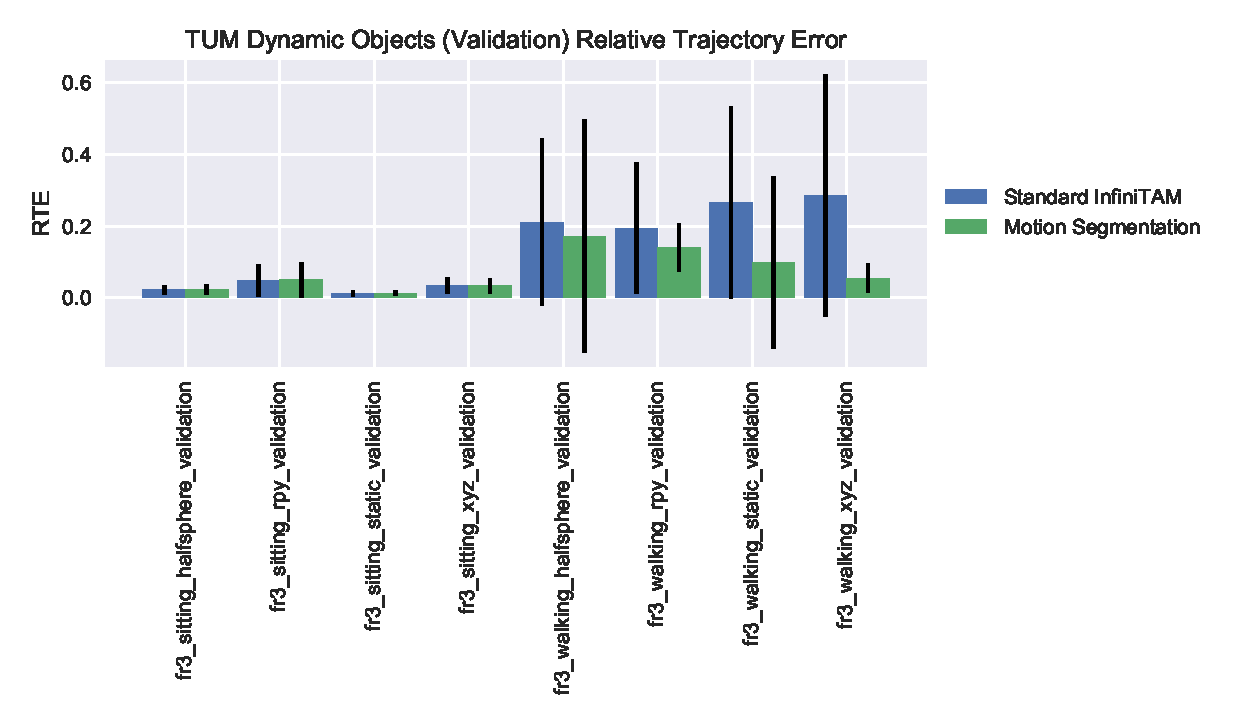
\includegraphics[width=\linewidth]{figures/moseg/rte_validation.eps}
  \caption[Motion Segmentation RTE Validation Set]
  {Relative Trajectory Error for the TUM Dynamic Scenes
    \textit{Validation} dataset.}
\end{figure}